\documentclass{article}

\def \lastexercisenumber{15}

% Hier befinden sich Pakete, die wir beinahe immer benutzen ...

\usepackage[utf8]{inputenc}

% Sprach-Paket:
\usepackage[ngerman]{babel}

% damit's nicht so, wie beim Grill aussieht:
\usepackage{fullpage}

% Mathematik:
\usepackage{amsmath, amssymb, amsfonts, amsthm}
\usepackage{bbm}
\usepackage{mathtools, mathdots}

% Makros mit mehereren Default-Argumenten:
\usepackage{twoopt}

% Anführungszeichen (Makro \Quote{}):
\usepackage{babel}

% if's für Makros:
\usepackage{xifthen}
\usepackage{etoolbox}

% tikz ist kein Zeichenprogramm (doch!):
\usepackage{tikz}

% bessere Aufzählungen:
\usepackage{enumitem}

% (bessere) Umgebung für Bilder:
\usepackage{graphicx, subfig, float}

% Umgebung für Code:
\usepackage{listings}

% Farben:
\usepackage{xcolor}

% Umgebung für "plain text":
\usepackage{verbatim}

% Umgebung für mehrerer Spalten:
\usepackage{multicol}

% "nette" Brüche
\usepackage{nicefrac}

% Spaltentypen verschiedener Dicke
\usepackage{tabularx}
\usepackage{makecell}

% Für Vektoren
\usepackage{esvect}

% (Web-)Links
\usepackage{hyperref}

% Zitieren & Literatur-Verzeichnis
\usepackage[style = authoryear]{biblatex}
\usepackage{csquotes}

% so ähnlich wie mathbb
%\usepackage{mathds}

% Keine Ahnung, was das macht ...
\usepackage{booktabs}
\usepackage{ngerman}
\usepackage{placeins}

% special letters:

\newcommand{\N}{\mathbb{N}}
\newcommand{\Z}{\mathbb{Z}}
\newcommand{\Q}{\mathbb{Q}}
\newcommand{\R}{\mathbb{R}}
\newcommand{\C}{\mathbb{C}}
\newcommand{\K}{\mathbb{K}}
\newcommand{\T}{\mathbb{T}}
\newcommand{\E}{\mathbb{E}}
\newcommand{\V}{\mathbb{V}}
\renewcommand{\S}{\mathbb{S}}
\renewcommand{\P}{\mathbb{P}}
\newcommand{\1}{\mathbbm{1}}

% quantors:

\newcommand{\Forall}{\forall \,}
\newcommand{\Exists}{\exists \,}
\newcommand{\ExistsOnlyOne}{\exists! \,}
\newcommand{\nExists}{\nexists \,}
\newcommand{\ForAlmostAll}{\forall^\infty \,}

% MISC symbols:

\newcommand{\landau}{{\scriptstyle \mathcal{O}}}
\newcommand{\Landau}{\mathcal{O}}


\newcommand{\eps}{\mathrm{eps}}

% graphics in a box:

\newcommandtwoopt
{\includegraphicsboxed}[3][][]
{
  \begin{figure}[!h]
    \begin{boxedin}
      \ifthenelse{\isempty{#1}}
      {
        \begin{center}
          \includegraphics[width = 0.75 \textwidth]{#3}
          \label{fig:#2}
        \end{center}
      }{
        \begin{center}
          \includegraphics[width = 0.75 \textwidth]{#3}
          \caption{#1}
          \label{fig:#2}
        \end{center}
      }
    \end{boxedin}
  \end{figure}
}

% braces:

\newcommand{\pbraces}[1]{{\left  ( #1 \right  )}}
\newcommand{\bbraces}[1]{{\left  [ #1 \right  ]}}
\newcommand{\Bbraces}[1]{{\left \{ #1 \right \}}}
\newcommand{\vbraces}[1]{{\left  | #1 \right  |}}
\newcommand{\Vbraces}[1]{{\left \| #1 \right \|}}
\newcommand{\abraces}[1]{{\left \langle #1 \right \rangle}}
\newcommand{\round}[1]{\bbraces{#1}}

\newcommand
{\floorbraces}[1]
{{\left \lfloor #1 \right \rfloor}}

\newcommand
{\ceilbraces} [1]
{{\left \lceil  #1 \right \rceil }}

% special functions:

\newcommand{\norm}  [2][]{\Vbraces{#2}_{#1}}
\newcommand{\diam}  [2][]{\mathrm{diam}_{#1} \: #2}
\newcommand{\diag}  [1]{\mathrm{diag} \: #1}
\newcommand{\dist}  [1]{\mathrm{dist} \: #1}
\newcommand{\mean}  [1]{\mathrm{mean} \: #1}
\newcommand{\erf}   [1]{\mathrm{erf} \: #1}
\newcommand{\id}    [1]{\mathrm{id} \: #1}
\newcommand{\sgn}   [1]{\mathrm{sgn} \: #1}
\newcommand{\supp}  [1]{\mathrm{supp} \: #1}
\newcommand{\arsinh}[1]{\mathrm{arsinh} \: #1}
\newcommand{\arcosh}[1]{\mathrm{arcosh} \: #1}
\newcommand{\artanh}[1]{\mathrm{artanh} \: #1}
\newcommand{\card}  [1]{\mathrm{card} \: #1}
\newcommand{\Span}  [1]{\mathrm{span} \: #1}
\newcommand{\Aut}   [1]{\mathrm{Aut} \: #1}
\newcommand{\End}   [1]{\mathrm{End} \: #1}
\newcommand{\ggT}   [1]{\mathrm{ggT} \: #1}
\newcommand{\kgV}   [1]{\mathrm{kgV} \: #1}
\newcommand{\ord}   [1]{\mathrm{ord} \: #1}
\newcommand{\grad}  [1]{\mathrm{grad} \: #1}
\newcommand{\ran}   [1]{\mathrm{ran} \: #1}
\newcommand{\graph} [1]{\mathrm{graph} \: #1}
\newcommand{\Inv}   [1]{\mathrm{Inv} \: #1}
\newcommand{\pv}    [1]{\mathrm{pv} \: #1}
\newcommand{\GL}    [1]{\mathrm{GL} \: #1}
\newcommand{\Mod}{\mathrm{Mod} \:}
\newcommand{\Th}{\mathrm{Th} \:}
\newcommand{\Char}{\mathrm{char}}
\newcommand{\At}{\mathrm{At}}
\newcommand{\Ob}{\mathrm{Ob}}
\newcommand{\Hom}{\mathrm{Hom}}
\newcommand{\orthogonal}[3][]{#2 ~\bot_{#1}~ #3}
\newcommand{\Rang}{\mathrm{Rang}}
\newcommand{\NIL}{\mathrm{NIL}}
\newcommand{\Res}{\mathrm{Res}}
\newcommand{\lxor}{\dot \lor}
\newcommand{\Div}{\mathrm{div} \:}
\newcommand{\meas}{\mathrm{meas} \:}

% fractions:

\newcommand{\Frac}[2]{\frac{1}{#1} \pbraces{#2}}
\newcommand{\nfrac}[2]{\nicefrac{#1}{#2}}

% derivatives & integrals:

\newcommandtwoopt
{\Int}[4][][]
{\int_{#1}^{#2} #3 ~\mathrm{d} #4}

\newcommandtwoopt
{\derivative}[3][][]
{
  \frac
  {\mathrm{d}^{#1} #2}
  {\mathrm{d} #3^{#1}}
}

\newcommandtwoopt
{\pderivative}[3][][]
{
  \frac
  {\partial^{#1} #2}
  {\partial #3^{#1}}
}

\newcommand
{\primeprime}
{{\prime \prime}}

\newcommand
{\primeprimeprime}
{{\prime \prime \prime}}

% Text:

\newcommand{\Quote}[1]{\glqq #1\grqq{}}
\newcommand{\Text}[1]{{\text{#1}}}
\newcommand{\fastueberall}{\text{f.ü.}}
\newcommand{\fastsicher}{\text{f.s.}}

% -------------------------------- %
% amsthm-stuff:

\theoremstyle{definition}

% numbered theorems
\newtheorem{theorem}{Satz}
\newtheorem{lemma}{Lemma}
\newtheorem{corollary}{Korollar}
\newtheorem{proposition}{Proposition}
\newtheorem{remark}{Bemerkung}
\newtheorem{definition}{Definition}
\newtheorem{example}{Beispiel}

% unnumbered theorems
\newtheorem*{theorem*}{Satz}
\newtheorem*{lemma*}{Lemma}
\newtheorem*{corollary*}{Korollar}
\newtheorem*{proposition*}{Proposition}
\newtheorem*{remark*}{Bemerkung}
\newtheorem*{definition*}{Definition}
\newtheorem*{example*}{Beispiel}

% Please define this stuff in project ("main.tex"):

% \def \lastexercisenumber {...}
% This will be 0 by default

% \setcounter{section}{...}
% This will be 0 by default
% and hence, completely ignored

\ifnum \thesection = 0
{\newtheorem{exercise}{Aufgabe}}
\else
{\newtheorem{exercise}{Aufgabe}[section]}
\fi

\ifdef
{\lastexercisenumber}
{\setcounter{exercise}{\lastexercisenumber}}

\newcommand{\solution}
{
    \renewcommand{\proofname}{Lösung}
    \renewcommand{\qedsymbol}{}
    \proof
}

\renewcommand{\proofname}{Beweis}

% -------------------------------- %
% environment zum einkasteln:

% dickere vertical lines
\newcolumntype
{x}
[1]
{!{\centering\arraybackslash\vrule width #1}}

% environment selbst (the big cheese)
\newenvironment
{boxedin}
{
  \begin{tabular}
  {
    x{1 pt}
    p{\textwidth}
    x{1 pt}
  }
  \Xhline
  {2 \arrayrulewidth}
}
{
  \\
  \Xhline{2 \arrayrulewidth}
  \end{tabular}
}

% -------------------------------- %
% MISC "Ein-Deutschungen"

\renewcommand
{\figurename}
{Abbildung}

\renewcommand
{\tablename}
{Tabelle}

% -------------------------------- %


\addbibresource{../../../Fundament-LaTeX/references.bib}

\graphicspath{{../../../Fundament-LaTeX/images/}}

\parindent 0pt

\title
{
  Numerik von Partiellen Differentialgleichungen: stationäre Probleme \\
  \vspace{4pt}
  \normalsize
  \textit{4. Übung am 25.11.2020}
}
\author
{
  Richard Weiss
  \and
  Florian Schager
  \and
  Christian Sallinger
  \and
  Fabian Zehetgruber
  \and
  Paul Winkler
  \and
  Christian Göth
}
\date{}

\begin{document}

\maketitle

% -------------------------------------------------------------------------------- %

\begin{exercise}

ToDo!

\end{exercise}

% -------------------------------------------------------------------------------- %

\begin{solution}

ToDo!

\end{solution}

% -------------------------------------------------------------------------------- %

% -------------------------------------------------------------------------------- %

\begin{exercise}

ToDo!

\end{exercise}

% -------------------------------------------------------------------------------- %

\begin{solution}

ToDo!

\end{solution}

% -------------------------------------------------------------------------------- %

% -------------------------------------------------------------------------------- %

\begin{exercise}

Verallgemeinern Sie Theorem 3.5 auf die Triangulierung eines beschränkten Lipschitz-Gebietes $\Omega \in \R^3$ mit Tetraedern.
Beweisen Sie dazu die Abschätzungen (3.20) und (3.21) für ein nicht-entartetes Tetraeder $T$.
Die Konstante $\sigma(T)$ wird dabei analog zu Aufgabe 11b definiert durch den Quotienten aus dem Durchmesser $h_T := \max \Bbraces{|x - y|: x, y \in T}$ von $T$ und dem Radius $\rho_T$ der größten Kugel, welche noch ganz in $T$ liegt, d.h.

\begin{align}
  \rho_T
  :=
  \sup \Bbraces{\rho > 0: \Exists x \in T \quad B(x, \rho) \subset T}.
\end{align}

\end{exercise}

% -------------------------------------------------------------------------------- %

\begin{solution}

\phantom{}

\includegraphicsunboxed{NumPDEs/NumPDEs - Theorem 3.5 (Approximation Theorem).png}

Die einzigen Teile im Beweis von Theorem 3.5 (Approximation Theorem), die nicht für den $\R^3$ funktionieren, sind die, wo Lemma 3.9 verwendet wird.

\includegraphicsunboxed{NumPDEs/NumPDEs - Lemma 3.9.png}

\begin{tcolorbox}[standard jigsaw, opacityback = 0]

\textbf{Lemma 3.9}
($\R^3$)
Für

\begin{align*}
  \hat T
  =
  T_\mathrm{ref}
  =
  \conv
  \Bbraces
  {
    \begin{pmatrix}
      0 \\ 0 \\ 0
    \end{pmatrix},
    \begin{pmatrix}
      1 \\ 0 \\ 0
    \end{pmatrix},
    \begin{pmatrix}
      0 \\ 1 \\ 0
    \end{pmatrix},
    \begin{pmatrix}
      0 \\ 0 \\ 1
    \end{pmatrix}
  }
\end{align*}

das Referenz-Element und $T = \conv \Bbraces{z_1, z_2, z_3, z_4} \subset \R^3$ ein nicht-degeneriertes Tetraeder, definieren wir

\begin{align*}
  \Phi_T:
  T_\mathrm{ref} \to T,
  x \mapsto z_1 + B x,
  \quad
  ~\text{wobei}~
  B := (z_2 - z_1, z_3 - z_1, z_4 - z_1) \in \R^{3 \times 3}.
\end{align*}

Dann gilt, dass $\abs{\det B} = 6 |T|$ und

\begin{align*}
  h_T / \sqrt{2} \leq \norm[F]{B} \leq \sqrt{3} h_T
  \quad
  \text{als auch}
  \quad
  \norm[F]{B^{-1}} \leq 3 C \rho_T^{-1},
\end{align*}

wobei $C > 0$ unabhängig von $T$ ist.

\end{tcolorbox}

\textbf{\textit{Beweis.}}
Es gilt, dass

\begin{align*}
  \norm[F]{B}^2
  =
  |z_2 - z_1|^2 + |z_3 - z_1|^2 + |z_4 - z_1|^2
  \leq
  3 h_T^2.
\end{align*}

Des weiteren

\begin{align*}
  \begin{rcases}
    |z_3 - z_2| \leq |z_3 - z_1| + |z_1 - z_2| \leq \sqrt{2} \pbraces{|z_3 - z_1|^2 + |z_1 - z_2|^2}^{1/2} \\
    |z_4 - z_2| \leq |z_4 - z_1| + |z_1 - z_2| \leq \sqrt{2} \pbraces{|z_4 - z_1|^2 + |z_1 - z_2|^2}^{1/2} \\
    |z_4 - z_3| \leq |z_4 - z_1| + |z_1 - z_3| \leq \sqrt{2} \pbraces{|z_4 - z_1|^2 + |z_1 - z_3|^2}^{1/2}
  \end{rcases}
  \leq
  \sqrt{2} \norm[F]{B}.
\end{align*}

Speziell, $h_T = \max \Bbraces{|z_2 - z_1|, |z_3 - z_1|, |z_3 - z_2|, |z_4 - z_1|, |z_4 - z_2|, |z_4 - z_3|} \leq \sqrt{2} \norm[F]{B}$.

\includegraphicsboxed{Ana3/Ana3 - Satz 4.4.1 (Koflächenformel).png}

Wir wenden die Koflächenformel auf $f(x,y,z) = z,\ |\nabla f(x,y,z)| = 1$ und $g(x,y,z) = 1$ an und berechnen

\begin{align*}
  |T_\mathrm{ref}|
  =
  \Int[T_\mathrm{ref}]{}{\lambda}
  = \Int[0][1]{\mathcal{H}^2(f^{-1}(h))}{h}
  \Int[0][1]{(1 - h)^2 / 2}{h}
  =
  \frac{1}{2} \Int[0][1]{1 - 2 h + h^2}{h}
  =
  \frac{1}{2} \pbraces{1 - 1 + \frac{1}{3}}
  =
  \frac{1}{6}.
\end{align*}

\includegraphicsboxed{Ana3/Ana3 - Satz 4.3.1 (Transformationsformel).png}

Die Transformationsformel gibt uns

\begin{align*}
  \frac{1}{6} \abs{\det B}
  =
  |T_\mathrm{ref}| \abs{\det B}
  =
  \Int[T_\mathrm{ref}]{\abs{\det D \Phi_T}}{x}
  =
  \Int[T]{}{x}
  =
  |T|
  >
  0.
\end{align*}

Also, $\abs{\det B} = 6 |T|$.
Insbesondere, ist $B^{-1}$ wohldefiniert.
Es gilt, dass

\begin{align*}
  B^{-1}
  =
  \frac{1}{\det B} \cof(B)^\top,
\end{align*}

wobei ja

\begin{align*}
  B
  =
  \begin{pmatrix}
    (z_2 - z_1)_1 & (z_3 - z_1)_1 & (z_4 - z_1)_1 \\
    (z_2 - z_1)_2 & (z_3 - z_1)_2 & (z_4 - z_1)_2 \\
    (z_2 - z_1)_3 & (z_3 - z_1)_3 & (z_4 - z_1)_3
  \end{pmatrix},
\end{align*}

und daher

\begin{multline*}
  \cof(B)^\top
  =
  \begin{pmatrix}
    +
    \det
    \begin{pmatrix}
      (z_3 - z_1)_2 & (z_4 - z_1)_2 \\
      (z_3 - z_1)_3 & (z_4 - z_1)_3
    \end{pmatrix}
    &
    -
    \det
    \begin{pmatrix}
      (z_2 - z_1)_2 & (z_4 - z_1)_2 \\
      (z_2 - z_1)_3 & (z_4 - z_1)_3
    \end{pmatrix}
    &
    +
    \det
    \begin{pmatrix}
      (z_2 - z_1)_2 & (z_3 - z_1)_2 \\
      (z_2 - z_1)_3 & (z_3 - z_1)_3
    \end{pmatrix}
    \\
    -
    \det
    \begin{pmatrix}
      (z_3 - z_1)_1 & (z_4 - z_1)_1 \\
      (z_3 - z_1)_3 & (z_4 - z_1)_3
    \end{pmatrix}
    &
    +
    \det
    \begin{pmatrix}
      (z_2 - z_1)_1 & (z_4 - z_1)_1 \\
      (z_2 - z_1)_3 & (z_4 - z_1)_3
    \end{pmatrix}
    &
    -
    \det
    \begin{pmatrix}
      (z_2 - z_1)_1 & (z_3 - z_1)_1 \\
      (z_2 - z_1)_3 & (z_3 - z_1)_3
    \end{pmatrix}
    \\
    +
    \det
    \begin{pmatrix}
      (z_3 - z_1)_1 & (z_4 - z_1)_1 \\
      (z_3 - z_1)_2 & (z_4 - z_1)_2
    \end{pmatrix}
    &
    -
    \det
    \begin{pmatrix}
      (z_2 - z_1)_1 & (z_4 - z_1)_1 \\
      (z_2 - z_1)_2 & (z_4 - z_1)_2
    \end{pmatrix}
    &
    +
    \det
    \begin{pmatrix}
      (z_2 - z_1)_1 & (z_3 - z_1)_1 \\
      (z_2 - z_1)_2 & (z_3 - z_1)_2
    \end{pmatrix}
  \end{pmatrix}.
\end{multline*}

Nachem $\dim \GL_3(\R) = 9 < \infty$, können wir statt der Frobeinius-Norm die äquivalente Norm $\norm{\cdot}$ verwenden.
Diese ist also nur um eine gleichmäßige Konstante $C > 0$ größer.

\begin{align*}
  \norm{B}
  :=
  \sum_{i,j=1}^3 |b_{ij}|,
  \quad
  \norm[F]{\cdot}
  \sim
  \norm{\cdot}
  \implies
  \Exists C > 0:
  \norm[F]{\cdot}
  \leq
  C \norm{\cdot}.
\end{align*}

Wir definieren die Seiten-Flächen des Tetraeders $T$.

\begin{align*}
  T_1 & := \conv \Bbraces{z_1, z_2, z_3} \\
  T_2 & := \conv \Bbraces{z_2, z_3, z_4} \\
  T_3 & := \conv \Bbraces{z_3, z_4, z_1} \\
  T_4 & := \conv \Bbraces{z_4, z_1, z_2}
\end{align*}

Das Flächenmaß $|A|$ einer Fläche $A$ ist immer kleiner gleich $|f(A)|$, dem Flächenmaß der orthogonal-projezierten Fläche $f(A)$.
Das basiert auf den folgenden beiden Resultaten aus \cite{Ana3} bzw. \cite{FAna1}.

\includegraphicsboxed{Ana3/Ana3 - Proposition 4.1.2.png}
\includegraphicsboxed{FAna1/FAna1 - orthogonale Projektion 4.png}

Damit erhalten wir folgende Abschätzungen, wenn $\pi$ eine orthogonale Projektion ist:

\begin{align*}
  |T_1| & \geq |\pi(T_1)| = \frac{1}{2} \det(\pi(z_3 - z_1), \pi (z_4 - z_1)) \\
  |T_3| & \geq |\pi(T_3)| = \frac{1}{2} \det(\pi(z_2 - z_1), \pi (z_4 - z_1)) \\
  |T_4| & \geq |\pi(T_4)| = \frac{1}{2} \det(\pi(z_2 - z_1), \pi (z_3 - z_1))
\end{align*}

Wir erhalten also folgende Abschätzung:

\begin{align*}
  & \norm{\cof(B)^\top}
  =
  \vbraces
  {
    \det
    \pbraces
    {
      \pi_{2, 3}(z_3 - z_1),
      \pi_{2, 3}(z_4 - z_1)
    }
  }
  +
  \vbraces
  {
    \det
    \pbraces
    {
      \pi_{2, 3}(z_2 - z_1),
      \pi_{2, 3}(z_4 - z_1)
    }
  }
  +
  \vbraces
  {
    \det
    \pbraces
    {
      \pi_{2, 3}(z_2 - z_1),
      \pi_{2, 3}(z_3 - z_1)
    }
  } \\
  +
  & \vbraces
  {
    \det
    \pbraces
    {
      \pi_{1, 3}(z_3 - z_1),
      \pi_{1, 3}(z_4 - z_1)
    }
  }
  +
  \vbraces
  {
    \det
    \pbraces
    {
      \pi_{1, 3}(z_2 - z_1),
      \pi_{1, 3}(z_4 - z_1)
    }
  }
  +
  \vbraces
  {
    \det
    \pbraces
    {
      \pi_{1, 3}(z_2 - z_1),
      \pi_{1, 3}(z_3 - z_1)
    }
  } \\
  +
  & \vbraces
  {
    \det
    \pbraces
    {
      \pi_{1, 2}(z_3 - z_1),
      \pi_{1, 2}(z_4 - z_1)
    }
  }
  +
  \vbraces
  {
    \det
    \pbraces
    {
      \pi_{1, 2}(z_2 - z_1),
      \pi_{1, 2}(z_4 - z_1)
    }
  }
  +
  \vbraces
  {
    \det
    \pbraces
    {
      \pi_{1, 2}(z_2 - z_1),
      \pi_{1, 2}(z_3 - z_1)
    }
  } \\
  & \leq
  2 |T_1| + 2 |T_3| + 2 |T_4| +
  2 |T_1| + 2 |T_3| + 2 |T_4| +
  2 |T_1| + 2 |T_3| + 2 |T_4| \\
  & \leq
  6 (|T_1| + |T_2| + |T_3| + |T_4|)
\end{align*}

Laut TUWEL-Forum, gilt folgende Formel.

\begin{align*}
  |T|
  =
  \frac{1}{3} \rho_T (|T_1| + |T_2| + |T_3| + |T_4|).
\end{align*}

Jetzt setzen wir alles zusammen.

\begin{multline*}
  \norm[F]{B^{-1}}
  \leq
  C \norm{B^{-1}}
  =
  C
  \norm
  {
    \frac{1}{\det B}
    \cof(B)^\top
  }
  =
  C
  \frac{1}{\abs{\det B}}
  \norm{\cof(B)^\top} \\
  =
  C
  \frac{1}{6 |T|}
  \norm{\cof(B)^\top}
  \leq
  C
  \frac
  {
    6 (|T_1| + |T_2| + |T_3| + |T_4|)
  }{
    6 \frac{1}{3} \rho_T (|T_1| + |T_2| + |T_3| + |T_4|)
  }
  =
  3 C \rho_T^{-1}
\end{multline*}

\end{solution}

% -------------------------------------------------------------------------------- %

% --------------------------------------------------------------------------------

\begin{exercise}

Für ein beschränktes Lipschitz-Gebiet $\Omega \subset \R^2$ definieren wir den Hilbertraum

\begin{align*}
  H(\curl, \Omega)
  :=
  \Bbraces{\xi \in [L^2(\Omega)]^2 | \curl \xi \in L^2(\Omega)}, 
  \quad
  (\xi, \zeta)_{H(\curl)}
  :=
  (\xi, \zeta)_{L^2(\Omega)} + (\curl \xi, \curl \zeta)_{L^2(\Omega)}, 
\end{align*}

mit $\curl \xi := \frac{\partial \xi_2}{\partial x} - \frac{\partial \xi_1}{\partial y}$ für $\xi(x, y) = (\xi_1(x, y), \xi_2(x, y))^\top$.
Weiter sei $X := H^1_0(\Omega) \times H(\curl, \Omega)$ ein Hilbert-Raum wie in Aufgabe 6.

Für ein $c \geq 0$ und $f \in L^2(\Omega)$ sei das folgende Variationsproblem gegeben: Finden Sie $(u, \xi) \in X$ sodass für alle $(v, \zeta) \in X$

\begin{align}
  \Int[\Omega]{(\nabla u - \xi) \cdot (\nabla v - \zeta)}{x}
  +
  c \Int[\Omega]{\xi \cdot \zeta}{x}
  +
  \Int[\Omega]{\curl \xi \curl \zeta}{x}
  =
  \Int[\Omega]{f v}{x}
\end{align}

\begin{enumerate}[label = \textbf{\alph*)}]

  \item Zeigen Sie mit Hilfe des Lemmas von Lax-Milgram, dass für $c > 0$ das Problem eine eindeutige Lösung hat.
  Verwenden Sie dazu am besten die Young Ungleichung $-ab \geq - \frac{\varepsilon}{2} a^2 - \frac{1}{2\varepsilon}b^2$ für geeignete $a, b \in \R$ und $\varepsilon > 0$.

  \item Es sei nun $c = 0$.
  Zeigen Sie durch geschicktes Wählen von $(u, \xi) \in X$, dass das Problem nicht koerziv ist.
  \textit{Hinweis}:
  Was gilt für $\curl \nabla u$?

  \item Begründen Sie mit den Funktionen $\xi_\varepsilon \in [H^1(\Omega)]^2$ definiert durch $\xi_\varepsilon(x, y) := (\sin(\frac{1}{\varepsilon}x), 0)^\top$ mit $\varepsilon > 0$, dass das Problem auf dem Produktraum $\hat{X} := H^1_0(\Omega) \times [H^1(\Omega)]^2$ mit $c > 0$ nicht koerziv und damit nicht wohlgestellt ist.

\end{enumerate}

\end{exercise}

% --------------------------------------------------------------------------------

\begin{solution}

\phantom{}

\begin{align*}
  \pbraces
  {
    \begin{pmatrix}
      u \\ \xi
    \end{pmatrix},
    \begin{pmatrix}
      v \\ \zeta
    \end{pmatrix}
  }_X
  & =
  (u, v)_{H^1(\Omega)}
  +
  (\xi, \zeta)_{H(\curl, \Omega)} \\
  & =
  (u, v)_{L^2(\Omega)}
  +
  (\nabla u, \nabla v)_{L^2(\Omega)}
  +
  (\xi, \zeta)_{L^2(\Omega)}
  +
  (\curl \xi, \curl \zeta)_{L^2(\Omega)}
\end{align*}

\begin{align*}
  \implies
  \norm[X]
  {
    \begin{pmatrix}
      u \\ \xi
    \end{pmatrix}
  }
  & =
  \pbraces
  {
    \begin{pmatrix}
      u \\ \xi
    \end{pmatrix},
    \begin{pmatrix}
      u \\ \xi
    \end{pmatrix}
  }_X^{1/2} \\
  & =
  \pbraces
  {
    (u, u)_{L^2(\Omega)}
    +
    (\nabla u, \nabla u)_{L^2(\Omega)}
    +
    (\xi, \xi)_{L^2(\Omega)}
    +
    (\curl \xi, \curl \xi)_{L^2(\Omega)}
  }^{1/2} \\
  & =
  \pbraces
  {
    \norm[L^2(\Omega)]{u}^2
    +
    \norm[L^2(\Omega)]{\nabla u}^2
    +
    \norm[L^2(\Omega)]{\xi}^2
    +
    \norm[L^2(\Omega)]{\curl \xi}^2
  }^{1/2}
\end{align*}

\begin{enumerate}[label = \textbf{\alph*)}]

  \item \phantom{}

  \begin{center}
    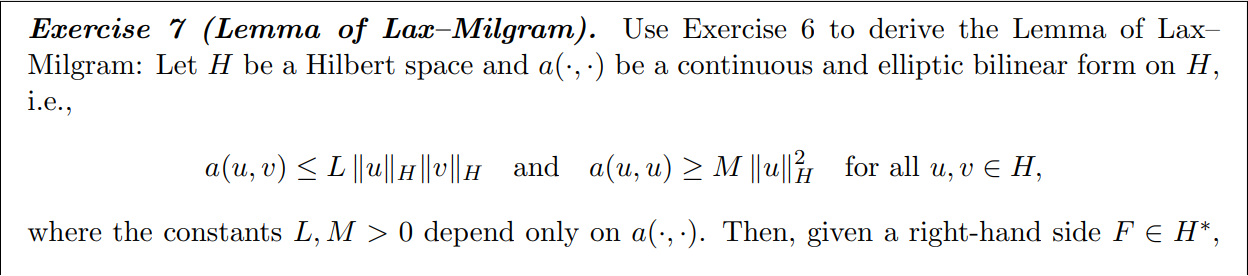
\includegraphics[width = 0.75 \textwidth]{NumPDEs/NumPDEs - Exercise 7.1 (Lemma of Lax-Milgram).png} \\
    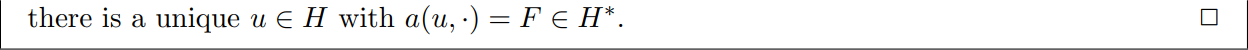
\includegraphics[width = 0.75 \textwidth]{NumPDEs/NumPDEs - Exercise 7.2 (Lemma of Lax-Milgram).png}
  \end{center}

  \begin{align*}
    a
    \pbraces
    {
      \begin{pmatrix}
        u \\ \xi
      \end{pmatrix},
      \begin{pmatrix}
        v \\ \zeta
      \end{pmatrix}
    }
    & :=
    \Int[\Omega]{(\nabla u - \xi) \cdot (\nabla v - \zeta)}{x}
    +
    c \Int[\Omega]{\xi \cdot \zeta}{x}
    +
    \Int[\Omega]{\curl \xi \curl \zeta}{x} \\
    F
    \begin{pmatrix}
      v \\ \xi
    \end{pmatrix}
    & :=
    \Int[\Omega]{f v}{x}
  \end{align*}

  \begin{enumerate}[label = \arabic*.]

    \item Stetigkeit von $a$:
    
    Auf dem $\R^3$ sind die Normen $\norm[1]{\cdot}$ und $\norm[2]{\cdot}$ äquivalent.
    Wir erhalten also eine Konstante $C > 0$, sodass $\norm[1]{\cdot} \leq C \norm[2]{\cdot}$.

    \begin{align*}
      \norm[1]{\cdot}
      \sim
      \norm[2]{\cdot}
      ~\text{auf $\R^3$}~
      \implies
      \Exists C > 0:
      \norm[1]{\cdot}
      \leq
      C
      \norm[2]{\cdot}
    \end{align*}

    \begin{align*}
      a
      \pbraces
      {
        \begin{pmatrix}
          u \\ \xi
        \end{pmatrix},
        \begin{pmatrix}
          v \\ \zeta
        \end{pmatrix}
      }
      & =
      \Int[\Omega]{(\nabla u - \xi) \cdot (\nabla v - \zeta)}{x}
      +
      c \Int[\Omega]{\xi \cdot \zeta}{x}
      +
      \Int[\Omega]{\curl \xi \curl \zeta}{x} \\
      & \stackrel
      {
        \mathrm{CSB}
      }{\leq}
      \norm[L^2(\Omega)]{\nabla u - \xi}
      \norm[L^2(\Omega)]{\nabla v - \zeta} \\
      & \quad
      +
      c
      \norm[L^2(\Omega)]{\xi}
      \norm[L^2(\Omega)]{\zeta}
      +
      \norm[L^2(\Omega)]{\curl \xi}
      \norm[L^2(\Omega)]{\curl \zeta} \\
      & \leq
      \pbraces
      {
        \norm[L^2(\Omega)]{\nabla u}
        +
        \norm[L^2(\Omega)]{\xi}
      }
      \pbraces
      {
        \norm[L^2(\Omega)]{\nabla u}
        +
        \norm[L^2(\Omega)]{\zeta}
      } \\
      & \quad
      +
      c
      \norm[L^2(\Omega)]{\xi}
      \norm[L^2(\Omega)]{\zeta}
      +
      \norm[L^2(\Omega)]{\curl \xi}
      \norm[L^2(\Omega)]{\curl \zeta} \\
      & \leq
      2 \max \Bbraces{1, c} \\
      & \quad
      \pbraces
      {
        \norm[H^1(\Omega)]{u}
        +
        \norm[L^2(\Omega)]{\xi}
        +
        \norm[L^2(\Omega)]{\curl \xi}
      } \\
      & \quad
      \pbraces
      {
        \norm[H^1(\Omega)]{v}
        +
        \norm[L^2(\Omega)]{\zeta}
        +
        \norm[L^2(\Omega)]{\curl \zeta}
      } \\
      & =
      2 \max \Bbraces{1, c} \\
      & \quad
      \norm[1]
      {
        \pbraces
        {
          \norm[H^1(\Omega)]{u},
          \norm[L^2(\Omega)]{\xi},
          \norm[L^2(\Omega)]{\curl \xi}
        }^\top
      } \\
      & \quad
      \norm[1]
      {
        \pbraces
        {
          \norm[H^1(\Omega)]{v},
          \norm[L^2(\Omega)]{\zeta},
          \norm[L^2(\Omega)]{\curl \zeta}
        }^\top
      } \\
      & \leq
      2 \max \Bbraces{1, c} C^2 \\
      & \quad
      \norm[2]
      {
        \pbraces
        {
          \norm[H^1(\Omega)]{u},
          \norm[L^2(\Omega)]{\xi},
          \norm[L^2(\Omega)]{\curl \xi}
        }^\top
      } \\
      & \quad
      \norm[2]
      {
        \pbraces
        {
          \norm[H^1(\Omega)]{v},
          \norm[L^2(\Omega)]{\zeta},
          \norm[L^2(\Omega)]{\curl \zeta}
        }^\top
      } \\
      & =
      2 \max \Bbraces{1, c} C^2 \\
      & \quad
      \pbraces
      {
        \norm[H^1(\Omega)]{u}^2
        +
        \norm[L^2(\Omega)]{\xi}^2
        +
        \norm[L^2(\Omega)]{\curl \xi}^2
      }^{1/2} \\
      & \quad
      \pbraces
      {
        \norm[H^1(\Omega)]{v}^2
        +
        \norm[L^2(\Omega)]{\zeta}^2
        +
        \norm[L^2(\Omega)]{\curl \zeta}^2
      }^{1/2} \\
      & =
      2 \max \Bbraces{1, c} C^2
      \norm[X]
      {
        \begin{pmatrix}
          u \\ \xi
        \end{pmatrix}
      }
      \norm[X]
      {
        \begin{pmatrix}
          v \\ \zeta
        \end{pmatrix}
      }
    \end{align*}

    \item Elliptizität von $a$:
    
    \includegraphicsunboxed{PDEs/PDEs_-_Satz_5-11_(Poincare-Ungleichung).png}

    Die Poincaré-Ungleichung von \cite{PDEs} liefert uns ein $C_p > 0:$

    \begin{align*}
      \norm[H^1(\Omega)]{u}^2
      =
      \norm[L^2(\Omega)]{u}^2
      +
      \norm[L^2(\Omega)]{\nabla u}^2
      \leq
      (C_p + 1)^2 \norm[L^2(\Omega)]{\nabla u}^2
      \implies
      \norm[L^2(\Omega)]{\nabla u}
      \geq
      \frac{1}{C_p + 1}
      \norm[H^1(\Omega)]{u}^2.
    \end{align*}

    In der folgenden Abschätzung verwenden wir die Young Ungleichung mit $\varepsilon \in \pbraces{\frac{1}{c + 1}, 1}$.
    
    \begin{align*}
      a
      \pbraces
      {
        \begin{pmatrix}
          u \\ \xi
        \end{pmatrix},
        \begin{pmatrix}
          u \\ \xi
        \end{pmatrix}
      }
      & =
      \Int[\Omega]{(\nabla u - \xi) \cdot (\nabla u - \xi)}{x}
      +
      c \Int[\Omega]{\xi \cdot \xi}{x}
      +
      \Int[\Omega]{\curl \xi \curl \xi}{x} \\
      & =
      \norm[L^2(\Omega)]{\nabla u - \xi}^2
      +
      c \norm[L^2(\Omega)]{\xi}^2
      +
      \norm[L^2(\Omega)]{\curl \xi}^2 \\
      & \geq
      \pbraces
      {
        \norm[L^2(\Omega)]{\nabla u}
        -
        \norm[L^2(\Omega)]{\xi}
      }^2
      +
      c \norm[L^2(\Omega)]{\xi}^2
      +
      \norm[L^2(\Omega)]{\curl \xi}^2 \\
      & =
      \norm[L^2(\Omega)]{\nabla u}^2
      -
      2
      \norm[L^2(\Omega)]{\nabla u}
      \norm[L^2(\Omega)]{\xi}
      +
      \norm[L^2(\Omega)]{\xi}^2
      +
      c
      \norm[L^2(\Omega)]{\xi}^2
      +
      \norm[L^2(\Omega)]{\curl \xi}^2 \\
      & \stackrel
      {
        \mathrm{Y}
      }{\geq}
      \norm[L^2(\Omega)]{\nabla u}^2
      -
      \varepsilon
      \norm[L^2(\Omega)]{\nabla u}^2
      -
      \frac{1}{\varepsilon}
      \norm[L^2(\Omega)]{\xi}^2
      +
      \norm[L^2(\Omega)]{\xi}^2
      +
      c
      \norm[L^2(\Omega)]{\xi}^2
      +
      \norm[L^2(\Omega)]{\curl \xi}^2 \\
      & =
      (1 - \varepsilon)
      \norm[L^2(\Omega)]{\nabla u}^2
      +
      \pbraces{1 + c - \frac{1}{\varepsilon}}
      \norm[L^2(\Omega)]{\xi}^2
      +
      \norm[L^2(\Omega)]{\curl \xi}^2 \\
      & \geq
      \frac{1 - \varepsilon}{(C_p + 1)^2}
      \norm[H^1(\Omega)]{\nabla u}^2
      +
      \pbraces{1 + c - \frac{1}{\varepsilon}}
      \norm[L^2(\Omega)]{\xi}^2
      +
      \norm[L^2(\Omega)]{\curl \xi}^2 \\
      & \geq
      \min
      \Bbraces
      {
        \frac{1 - \varepsilon}{(C_p + 1)^2},
        1 + c - \frac{1}{\varepsilon},
        1
      }
      \pbraces
      {
        \norm[H^1(\Omega)]{\nabla u}^2
        +
        \norm[L^2(\Omega)]{\xi}^2
        +
        \norm[L^2(\Omega)]{\curl \xi}^2
      } \\
      & =
      \min
      \Bbraces
      {
        \frac{1 - \varepsilon}{(C_p + 1)^2},
        1 + c - \frac{1}{\varepsilon},
        1
      }
      \norm[X]
      {
        \begin{pmatrix}
          u \\ \xi
        \end{pmatrix}
      }^2
    \end{align*}

    Wir sind fertig, weil $c > 0$.

    \item Stetigkeit von $F$:
    
    \begin{align*}
      F
    \begin{pmatrix}
      v \\ \xi
    \end{pmatrix}
    =
    \Int[\Omega]{f v}{x}
    \stackrel
    {
      \mathrm{CSB}
    }{\leq}
    \norm[L^2(\Omega)]{f}
    \norm[L^2(\Omega)]{v}
    \leq
    \norm[L^2(\Omega)]{f}
    \norm[X]
    {
      \begin{pmatrix}
        v \\ \xi
      \end{pmatrix}  
    }
    \end{align*}

  \end{enumerate}

\end{enumerate}

\end{solution}

% --------------------------------------------------------------------------------

% --------------------------------------------------------------------------------

\begin{exercise}

\phantom{}

\begin{enumerate}[label = \textbf{\alph*)}]

  \item Es sei $\Omega = (0,1), t >0, f \in L^2(\Omega)$, und $X := H^1_D(\Omega) \times H^1_D(\Omega)$ mit $H^1_D(\Omega) := \Bbraces{u \in H^1(\Omega) | u(0) = 0}$.
  Das Problem des Timoshenko Balkens lautet:
  Gesucht ist $(w, \beta) \in X$ sodass für alle $(v, \delta) \in X$

  \begin{align}
    \Int[\Omega]{\beta^\prime \delta^\prime}{x}
    +
    \frac{1}{t^2} \Int[\Omega]{(w^\prime - \beta)(v^\prime - \delta)}{x}
    =
    \Int[\Omega]{f v}{x}.
  \end{align}

  Zeigen Sie, dass das Problem eindeutig lösbar ist. Wie verhält sich die Konstante in Cea's Lemma wenn $t \to 0$?
  \textit{Hinweis}:
  Verwenden Sie wie in Aufgabe 19 die Young Ungleichung für den gemischten Term sowie die Friedrich Ungleichung.

  \item Sei nun $\Omega \subset \R^2$ und $X := H^1_D(\Omega) \times [H^1_D(\Omega)]^2$.
  Betrachten Sie die Reissner-Mindlin Platte als zweidimiensionale Erweiterung des Timoshenko Balkens beschrieben durch das Problem:
  Gesucht ist $(w, \beta) \in X$ sodass für alle $(v, \delta) \in X$

  \begin{align}
    \Int[\Omega]{\epsilon(\beta):\epsilon(\delta)}{x}
    +
    \frac{1}{t^2} \Int[\Omega]{(\nabla w - \beta) \cdot (\nabla v - \delta)}{x}
    =
    \Int[\Omega]{f v}{x},
  \end{align}

  wobei $\epsilon(\beta) := 0.5 (\nabla \beta + (\nabla \beta)^\top)$ der symmetrische Gradient ist.
  Untersuchen Sie mit dem zur Verfügung gestellten Jupyter-File das Konvergenzverhalten für lineare Elemente bei verschiedenen Dickenparametern, $t \in \Bbraces{1, 0.1, 0.01, 0.001}$.
  Was beobachten Sie?
  Wie ändert sich das Verhalten für quadratisch finite Elemente?

\end{enumerate}

\end{exercise}

% --------------------------------------------------------------------------------

\begin{solution}

\phantom{}

\begin{enumerate}[label = \textbf{\alph*)}]

  \item Wir wollen wieder Exercise 7 (Lemma of Lax-Milgram) anwenden, diesmal mit

  \begin{align*}
    a
    \pbraces
    {
      \begin{pmatrix}
        w \\ \beta
      \end{pmatrix},
      \begin{pmatrix}
        v \\ \xi
      \end{pmatrix}
    }
    :=
    \Int[\Omega]{\beta^\prime \delta^\prime}{x}
    +
    \frac{1}{t^2} \Int[\Omega]{(w^\prime - \beta)(v^\prime - \delta)}{x},
    \quad
    F
    \begin{pmatrix}
      v \\ \delta
    \end{pmatrix}
    :=
    \Int[\Omega]{f v}{x}.
  \end{align*}

  \begin{enumerate}[label = \arabic*.]

    \item Schritt (Stetigkeit von $a$):
    
    Auf dem $\R^2$ sind die Normen $\norm[1]{\cdot}$ und $\norm[2]{\cdot}$ äquivalent.
    Wir erhalten also eine Konstante $C > 0$, sodass $\norm[1]{\cdot} \leq C \norm[2]{\cdot}$.

    \begin{align*}
      \norm[1]{\cdot}
      \sim
      \norm[2]{\cdot}
      ~\text{auf $\R^2$}~
      \implies
      \Exists C > 0:
      \norm[1]{\cdot}
      \leq
      C
      \norm[2]{\cdot}
    \end{align*}

    Vorausschauend auf das Lemma 1.6 (Céa), definieren wir noch die Konstante

    \begin{align*}
      \beta_t
      :=
      2 \max \Bbraces{1, \frac{1}{t^2}} C.
    \end{align*}

    \begin{align*}
      a
      \pbraces
      {
        \begin{pmatrix}
          w \\ \beta
        \end{pmatrix},
        \begin{pmatrix}
          v \\ \xi
        \end{pmatrix}
      }
      & =
      \Int[\Omega]{\beta^\prime \delta^\prime}{x}
      +
      \frac{1}{t^2} \Int[\Omega]{(w^\prime - \beta)(v^\prime - \delta)}{x} \\
      & \stackrel
      {
        \mathrm{CSB}
      }{\leq}
      \norm[L^2(\Omega)]{\beta^\prime}
      \norm[L^2(\Omega)]{\delta^\prime}
      +
      \frac{1}{t^2}
      \norm[L^2(\Omega)]{w^\prime - \beta}
      \norm[L^2(\Omega)]{v^\prime - \delta} \\
      & \leq
      \norm[L^2(\Omega)]{\beta^\prime}
      \norm[L^2(\Omega)]{\delta^\prime}
      +
      \frac{1}{t^2}
      \pbraces
      {
        \norm[L^2(\Omega)]{w^\prime}
        \norm[L^2(\Omega)]{\beta}
      }
      \pbraces
      {
        \norm[L^2(\Omega)]{v^\prime}
        \norm[L^2(\Omega)]{\delta}
      } \\
      & \leq
      2 \max \Bbraces{1, \frac{1}{t^2}}
      \pbraces
      {
        \norm[L^2(\Omega)]{w^\prime}
        \norm[L^2(\Omega)]{\beta}
      }
      \pbraces
      {
        \norm[L^2(\Omega)]{v^\prime}
        \norm[L^2(\Omega)]{\delta}
      } \\
      & = \cdots \leq
      2 \max \Bbraces{1, \frac{1}{t^2}} C
      \pbraces
      {
        \norm[L^2(\Omega)]{w^\prime}^2
        \norm[L^2(\Omega)]{\beta}^2
      }^{1/2}
      \pbraces
      {
        \norm[L^2(\Omega)]{v^\prime}^2
        \norm[L^2(\Omega)]{\delta}^2
      }^{1/2} \\
      & =
      \beta_t
      \norm[X]
      {
        \begin{pmatrix}
          w \\ \beta
        \end{pmatrix}
      }
      \norm[X]
      {
        \begin{pmatrix}
          v \\ \delta
        \end{pmatrix}
      }
    \end{align*}

    \item Schritt (Elliptizität von $a$):
    
    \begin{enumerate}[label = \arabic*.]

      \item Hilfs-Ungleichung (Friedrich):

      \begin{center}
        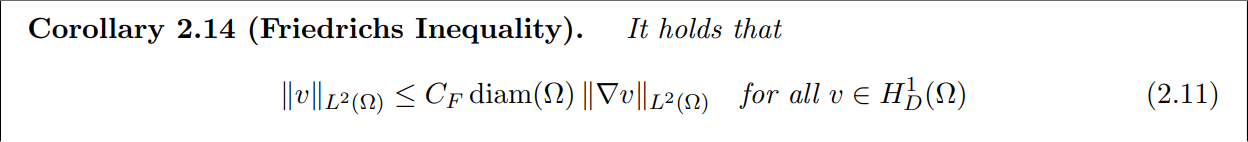
\includegraphics[width = 0.75 \textwidth]{NumPDEs/NumPDEs - Corollary 2.14.1 (Friedrichs Inequality).png} \\
        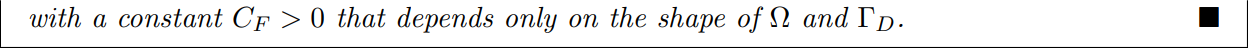
\includegraphics[width = 0.75 \textwidth]{NumPDEs/NumPDEs - Corollary 2.14.2 (Friedrichs Inequality).png}
      \end{center}

      \begin{align*}
        \implies
        \norm[H^1(\Omega)]{v}^2
        =
        \norm[L^2(\Omega)]{v}
        +
        \norm[L^2(\Omega)]{\nabla v}
        \stackrel
        {
          \mathrm{F}
        }{\leq}
        (
          C_F
          \underbrace{\diam \Omega}_1
          +
          1
        )^2
        \norm[L^2(\Omega)]{v^\prime}^2
      \end{align*}

      \item Hilfs-Ungleichung (Young):
      
      Dabei wollen wir $\varepsilon_t$ wie folgt wählen.

      \begin{align*}
        \varepsilon_t
        \in
        \pbraces
        {
          \frac{1}
          {
            1
            +
            \frac{t^2}{(C_F + 1)^2}
          },
          1
        }
        \neq
        \emptyset
      \end{align*}

      Das Intervall ist dabei nicht die leere Menge, weil $t > 0$ und daher

      \begin{align*}
        1 < 1 + \frac{t^2}{(C_F + 1)^2}.
      \end{align*}

    \end{enumerate}

    Vorausschauend auf das Lemma 1.6 (Céa), definieren wir noch die Konstante

    \begin{align*}
      \alpha_t
      :=
      \min
      \Bbraces
      {
        \frac{1}{(C_F + 1)^2}
        +
        \frac{1}{t^2}
        \pbraces
        {
          1 - \frac{1}{\varepsilon_t}
        },
        \frac
        {
          1 - \varepsilon_t
        }{
          t^2 (C_F + 1)^2
        }
      }.
    \end{align*}

    \begin{align*}
      a
      \pbraces
      {
        \begin{pmatrix}
          w \\ \beta
        \end{pmatrix},
        \begin{pmatrix}
          w \\ \beta
        \end{pmatrix}
      }
      & =
      \norm[L^2(\Omega)]{\beta^\prime}^2
      +
      \frac{1}{t^2}
      \Int[\Omega]{\abs{w^\prime - \beta}^2}{x} \\
      & =
      \norm[L^2(\Omega)]{\beta^\prime}^2
      +
      \frac{1}{t^2}
      \pbraces
      {
        \norm[L^2(\Omega)]{w^\prime}^2
        +
        \Int[\Omega]{- 2 w^\prime \beta}{x}
        +
        \norm[L^2(\Omega)]{\beta}^2
      } \\
      & \stackrel
      {
        \mathrm{Y}
      }{\geq}
      \norm[L^2(\Omega)]{\beta^\prime}^2
      +
      \frac{1}{t^2}
      \pbraces
      {
        \norm[L^2(\Omega)]{w^\prime}^2
        +
        \Int[\Omega]{- \varepsilon_t \abs{w^\prime}^2}{x}
        +
        \Int[\Omega]{- \frac{1}{\varepsilon_t} \abs{\beta}^2}{x}
        +
        \norm[L^2(\Omega)]{\beta}^2
      } \\
      & =
      \norm[L^2(\Omega)]{\beta^\prime}^2
      +
      \frac{1}{t^2}
      \pbraces
      {
        (1 - \varepsilon_t)
        \norm[L^2(\Omega)]{w^\prime}^2
        +
        \pbraces
        {
          1 - \frac{1}{\varepsilon_t}
        }
        \norm[L^2(\Omega)]{\beta}^2
      } \\
      & \stackrel
      {
        \mathrm{F}
      }{\geq}
      \frac{1}{(C_F + 1)^2}
      \norm[H^2(\Omega)]{\beta}^2
      +
      \frac{1}{t}
      \pbraces
      {
        \frac{1 - \varepsilon_t}{(C_F + 1)^2}
        \norm[H^1(\Omega)]{w}^2
        +
        \pbraces
        {
          1 - \frac{1}{\varepsilon_t}
        }
        \norm[H^1(\Omega)]{\beta}^2
      } \\
      & =
      \pbraces
      {
        \frac{1}{(C_F + 1)^2}
        +
        \frac{1}{t^2}
        \pbraces
        {
          1 - \frac{1}{\varepsilon_t}
        }
      }
      \norm[H^1(\Omega)]{\beta}^2
      +
      \frac{1 - \varepsilon_t}{t^2 (C_F + 1)^2}
      \norm[H^1(\Omega)]{w}^2 \\
      & \geq
      \min
      \Bbraces
      {
        \frac{1}{(C_F + 1)^2}
        +
        \frac{1}{t^2}
        \pbraces
        {
          1 - \frac{1}{\varepsilon_t}
        },
        \frac
        {
          1 - \varepsilon_t
        }{
          t^2 (C_F + 1)^2
        }
      }
      \pbraces
      {
        \norm[H^1(\Omega)]{w}^2
        +
        \norm[H^1(\Omega)]{\beta}^2
      } \\
      & =
      \alpha_t
      \norm[X]
      {
        \begin{pmatrix}
          w \\ \beta
        \end{pmatrix}
      }^2
    \end{align*}

    \item Schritt (Stetigkeit von $F$):
    
    \begin{align*}
      F
      \begin{pmatrix}
        v \\ \delta
      \end{pmatrix}
      =
      \Int[\Omega]{f v}{x}
      \stackrel
      {
        \mathrm{CSB}
      }{\leq}
      \norm[L^2(\Omega)]{f}
      \norm[L^2(\Omega)]{v}
      \leq
      \norm[L^2(\Omega)]{f}
      \norm[X]
      {
        \begin{pmatrix}
          v \\ \delta
        \end{pmatrix}
      }
    \end{align*}

  \end{enumerate}

  \includegraphicsunboxed{NumPDEs/NumPDEs - Lemma 1.6 (Céa).png}

  Der Quotient in Lemma 1.6 (Céa) divergiert.

  \begin{align*}
    \beta_t
    & =
    2 \max \Bbraces{1, \frac{1}{t^2}} C
    \xrightarrow{t \to 0}
    \infty, \\
    \alpha_t
    & =
    \min
    \Bbraces
    {
      \frac{1}{(C_F + 1)^2}
      +
      \frac{1}{t^2}
      \pbraces
      {
        1 - \frac{1}{\varepsilon_t}
      },
      \frac
      {
        1 - \varepsilon_t
      }{
        t^2 (C_F + 1)^2
      }
    }
    \leq
    \frac
    {
      1 - \varepsilon_t
    }{
      t^2 (C_F + 1)^2
    }
    \leq
    \frac
    {
      1
      -
      \frac{1}
      {
        1
        +
        \frac{t^2}{(C_F + 1)^2}
      }
    }{
      t^2 (C_F + 1)^2
    } \\
    & =
    \frac
    {
      1 + \frac{t^2}{(C_f + 1)^2} - 1
    }{
      \pbraces
      {
        1 + \frac{t^2}{(C_F + 1)^2}
      }
      t^2 (C_F + 1)^2
    }
    =
    \frac{1}
    {
      (C_F + 1)^2
      \pbraces
      {
        (C_F + 1)^2 + t^2
      }
    }
    \xrightarrow{t \to 0}
    \frac{1}{(C_F + 1)^4} \\
    \implies
    \frac{\beta_t}{\alpha_t}
    & \xrightarrow{t \to 0}
    \infty
  \end{align*}

  Die Fehlerschranke (d.h. die rechte Seite von (1.20)) kann also beliebig groß werden.
  Somit können wir Lemma 1.6 (Céa) nicht anwenden, um den FEM-Fehler sinnvoll abzuschätzen.

\end{enumerate}

\end{solution}

% --------------------------------------------------------------------------------


\printbibliography

\end{document}
